% Artyom Voronin
%  __  __           _      _ 
% |  \/  | ___   __| | ___| |
% | |\/| |/ _ \ / _` |/ _ \ |
% | |  | | (_) | (_| |  __/ |
% |_|  |_|\___/ \__,_|\___|_|
%                            
% Brno, 2020

\documentclass[class=article, crop=false]{standalone}
\usepackage[subpreambles=true]{standalone}

\usepackage{subcaption}
\usepackage{caption}
\usepackage{sectsty}
\usepackage{graphicx}
\graphicspath{{img/}{../img/}{../../img/}}
\usepackage{listings}
\lstset{language=Python}
\usepackage{hyperref}
\usepackage{amsmath}
\usepackage{import}
\usepackage{subfiles}
\usepackage[utf8]{inputenc}
\usepackage[english]{babel}

%\usepackage[square, numbers]{natbib}
%\bibliographystyle{unsrtnat}
%\usepackage[nottoc]{tocbibind}

%\usepackage{biblatex}
%\addbibresource{citations.bib} %usage \cite{test}
% Margins
% 
\topmargin=-0.45in
\evensidemargin=0in
\oddsidemargin=0in
\textwidth=6.5in
\textheight=9.0in
\headsep=0.25in

%\title{Models}
%\author{Artyom Voronin} 
%\date{}

\begin{document}
%\tableofcontents

% -------------------------------------------------------
% Section
% -------------------------------------------------------
\section{System modeling}

\paragraph{First Principles} (White-Box) \\
% TODO Isermann Fault Detection str 72
Simplification, Liniarization, Reduction, Parameter Estimation. \\
SimScape (Physical modeling), Simulink (Differential equations).

\paragraph{Data-Driven modeling}(Black-Box) \\ % In many cases better for prediction
% TODO Isermann Fault Detection str 72
Measurements, Identification.

% Nonlinear dynamic modeling  Isermann FDS str. 84

\subsection{Pneumatic piston system overview}
%\begin{figure}[h!]
%    \centering
%    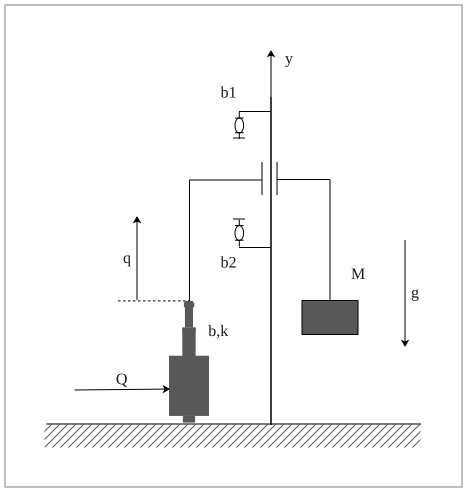
\includegraphics[width=0.5\textwidth]{model_draw_vec.png}
%    \caption{Schematic model}
%    \label{fig:model_draw}
%\end{figure}


% -------------------------------------------------------
% 
% -------------------------------------------------------

\subsection{Mechanical assembly}
\subsubsection{Equation of motion}

The motion of the pneumatic piston mechanism describes in terms of the
general 1dof dynamical equation \ref{eq:1dof}. 

\begin{equation}
    m\ddot{x} + b\dot{x} + kx = u
    \label{eq:1dof}
\end{equation}

%\begin{equation*}
%    \ddot{x} +\frac{b}{m}\dot{x} + \frac{k}{m}x = \frac{1}{m}u
%\end{equation*}
%
%\begin{equation*}
%    \ddot{x} +2\delta\dot{x} + \Omega^2x = \frac{1}{m}u
%\end{equation*}
%
%where $\delta = \frac{b}{2m}$ is damping and $\Omega = \sqrt{\frac{k}{m}}$
%is natural frequency of system.
%\begin{equation*}
%    \ddot{x} +2\zeta\Omega\dot{x} + \Omega^2x = \frac{1}{m}u
%\end{equation*}
%where $\zeta = \frac{b}{2\sqrt{km}}$ is damping ratio.


In the case of the pneumatic piston, the equation \ref{eq:1dof}
transforms into an equation \ref{eq:mechanical}.

\begin{equation}
    (M + M_L) \ddot{x} + F_{damp} + F_g + F_{hs}  = F_p
    \label{eq:mechanical}
\end{equation}

Where $M$ represents a mass of the all moveable part of the piston,
$M_L$ is load mass, $F_g$ gravity force acting to mechanical moving assembly,
$F_{hs}$ - models endpoints (hard stop),
$F_{damp}$ represents shock absorbers acted at endpoints,
$F_{p}$ is a force produced by the pneumatic piston \ref{eq:pneum}.

\begin{equation}
    F_p = P_A S_A - P_B S_B - P_0 S_0
    \label{eq:pneum}
\end{equation}

\subsubsection{Hard stop}
Hard stop can be represented as spring and dumps:

\begin{align}
    F_{HS} =
    \begin{cases}
        K_p(x-g_p) + D_pv & \text{for } x \ge g_p \\
        0 & \text{for } g_n < x < g_p \\
        K_n(x-g_n) + D_nv & \text{for } x \le g_n \\
    \end{cases}
\end{align}


Possible parameters: \\
\begin{tabular}{ |c|c|c| }
    \hline
    $K_p$ & $10^6$ & $[kg/s^2]$  \\
    $K_n$ & $10^6$ & $[kg/s^2]$  \\
    $D_p$ & $350$  & $[kg/s]$    \\
    $D_n$ & $350$  & $[kg/s]$    \\
    $g_n$ & $0  $  & $[m]$       \\
    $g_p$ & $0.2$  & $[m]$       \\
    \hline
\end{tabular}

\subsubsection{Shock Absorbers}

\subsection{Pressure model}

\begin{tabular}{ |c|c|c| }
    \hline
    $p_A, p_B$              & $Pa$              & pressure in chamber A, B \\
    $\dot{m_A}, \dot{m_B}$  & $kg \cdot s^{-1}$ & mass flow on way to chamber A, B \\
    $S_A, S_B$              & $m^2$             & piston area  \\
    $V_A, V_B$              & $m^3$             & volume of chamber A,B \\
    $V_{0A}, V_{0B}$        & $m^3$             & "dead" volume of chamber A,B \\
    $m$                     & $kg$              & piston mass\\
    $F_{load}$              & $N$               & load \\
    $x$                     & $m$               & piston position \\
    $l$                     & $m$               & maximum piston position \\
    \hline
\end{tabular}



\paragraph{Isothermal model}
\begin{align}
    m = \rho V \\
    \dot{m} = \dot{\rho} V + \rho \dot{V}
\end{align}

Applying \ref{eq:equation_of_state}:
\begin{align}
    \rho = \frac{p}{RT} \\
    \dot{\rho} = \frac{\dot{p}}{RT} 
\end{align}

Finally get \ref{eq:pressure1}:
\begin{align}
    \dot{p} = - \frac{p}{V}\dot{V} + \frac{RT}{V}\dot{m}
    \label{eq:pressure1}
\end{align}

\paragraph{Adiabatic model} 
For simple adiabatic model following equation can be used
\ref{eq:pressure_adiabatic_simple_model}:

\begin{align}
    \dot{p} = - \frac{\gamma p}{V}\dot{V} + \frac{\gamma RT}{V}\dot{m}
    \label{eq:pressure_adiabatic_simple_model}
\end{align}

\begin{align}
    \dot{p_A} = \frac{\gamma}{S_A x + V_{0A}} \left(- p_A S_A\dot{x} + RT_A\dot{m_A}
    \right)
\end{align}

\begin{align}
    \dot{p_B} = \frac{\gamma}{S_B (l-x) + V_{0B}} \left(p_B S_B\dot{x} + RT_B\dot{m_B}
    \right)
\end{align}

Volumes of chambers:
\begin{align}
    V_A = S_A x + V_{0A} \\
    V_B = S_B (l-x) + V_{0B} \\
    \dot{V}_A = S_A \dot{x} \\
    \dot{V}_B = - S_B \dot{x}
\end{align}

$T_A, T_B$ calculated from \ref{eq:equation_of_state}, or in adiabatic
model this parameters can remain constant same as atmospheric temperature.




\subsection{General physical principles}

\subsubsection{Thermodynamics}
\begin{tabular}{ |c|c|c| }
    \hline
    $p$                     & $Pa$              & pressure \\
    $V$                     & $m^3$             & volume \\
    $m$                     & $kg$              & mass \\
    $n$                     & $mol$             & amount of substance \\
    $R$                     & $Jkg^{-1}K^{-1}$  & ideal gas constant \\
    $r$                     & $Jkg^{-1}K^{-1}$  & mass-specific gas constant \\
    $T$                     & $K$               & temperature \\
    $S$                     & $m$               & area \\
    $z$                     & $m$               & height \\
    $w$                     & $ms^{-1}$         & flow speed \\
    $H$                     & $J$               & enthalpy \\
    $\nu$                   & $m^3kg^{-1}$      & specific volume \\
    $Q$                     & $J$               & heat shared with
                                                    environment \\
    $W_T$                   & $J$               & work \\
    $c_p$                   & $Jkg^{-1}K^{-1}$  & is the specific heat
                                                    at constant pressure \\
    $c_v$                   & $Jkg^{-1}K^{-1}$  & is the specific heat at constant volume\\
    $g=9.81$                & $ms^{-2}$         & gravity acceleration \\
    $\gamma=1.4\text{(air)}$& $-$               & heat capacity ratio
                                                    (isentropic expansion factor)\\
    \hline
\end{tabular}

\subsubsection{Equation of state}
Generally $pV=nRT$ but for air purpose were $r=\frac{pv}{T}=R=287.1 [Jkg^{-1}K^{-1}]$
following equation can be used \ref{eq:equation_of_state}:
\begin{align}
    pV = mrT
    \label{eq:equation_of_state}
\end{align} 

\subsubsection{Isothermal process}
Used in some papers \ref{eq:isothermal_process}:
\begin{align}
    p_1 V_1 = p_2 V_2 = const
    \label{eq:isothermal_process}
\end{align}
\subsubsection{Adiabatic process}

Adiabatic process \ref{eq:adiobatic_process}:
\begin{align}
     p_1V_1^{\gamma} =  p_2V_2^{\gamma} = const
    \label{eq:adiobatic_process}
\end{align}

Heat capacity ratio:
\begin{align}
    \gamma = \frac{c_p}{c_v}
\end{align}

Mayer's relation:
\begin{align}
    c_p = c_v + R
\end{align}

\subsubsection{Bernoulli's principle}
Bernoulli's principle \ref{eq:bernoullis_principle}:
\begin{align}
    H_1 + \frac{mw_1^2}{2} + mgz_1 + Q = H_2 + \frac{mw_2^2}{2} + mgz_w +
    W_T
    \label{eq:bernoullis_principle}
\end{align}

\begin{align}
    H_1- H_2 = -\int_1^2 V dp = c_p(T_1-T_2) = c_p T_1(1-\frac{T_2}{T_1})
    \label{eq:etalpi_sub}
\end{align}

Differential form:
\begin{align}
    \nu dp + w dw + g dz + dw_T = 0
\end{align}


\subsubsection{Fluid mechanics}
\begin{tabular}{ |c|c|c| }
    \hline
    $\dot{m}$                   & $kgs^{-1}$  & mass flow \\
    $c$                         & $ms^{-2}$   & speed of sound \\
    $w_k$                       & $ms^{-2}$   & critical flow velocity \\
    $\psi$                      & $-$         & flow coefficient \\
    $\psi_{max}$                & $-$         & critical flow coefficient \\
    $\beta$                     & $-$         & ration of pressure
                                                    differential \\
    $\beta_k$                   & $-$         & critical ratio of pressure
                                                    differential \\

    \hline
\end{tabular}

Continuity equation \ref{eq:continuity_equation}: 
\begin{align}
    \dot{m} = S_1 w_1 \rho_1 = S_2 w_2 \rho_2 = const
    \label{eq:continuity_equation}
\end{align}

\subsubsection{Air expansion from tank}
Assuming $W_T = 0, z_1 = z_2, Q = 0$ conditions and combine with
\ref{eq:bernoullis_principle} we will get \ref{eq:w2} equation:

\begin{align}
    w_2 = \sqrt{2(H_1 - H_2)}
    \label{eq:w2}
\end{align}

\begin{align}
    w_2 =
    \sqrt{2RT_1(\frac{\gamma}{\gamma-1})(1-(\frac{p_2}{p_1})^\frac{\gamma-1}{\gamma})}
    \label{eq:w2_final}
\end{align}

\begin{align}
    \rho_2 = \frac{p_1}{RT_1} (\frac{p_2}{p_1})^{\frac{1}{\gamma}}
    \label{eq:rho2}
\end{align}

Together \ref{eq:continuity_equation} \ref{eq:w2_final} \ref{eq:rho2}:
\begin{align}
    \dot{m} = S p_1 \sqrt{\frac{2}{RT_1}} \cdot
    \sqrt{\frac{\gamma}{\gamma-1}\left(\left(\frac{p_2}{p_1}\right)^\frac{2}{\gamma} -
    \left(\frac{p_2}{p_1}\right)^\frac{\gamma + 1}{\gamma}\right)}
    \label{}
\end{align}

where: 
\begin{align}
    \psi\left(\frac{p_2}{p_1}\right) =  
    \sqrt{\frac{\gamma}{\gamma-1}\left(\left(\frac{p_2}{p_1}\right)^\frac{2}{\gamma} -
    \left(\frac{p_2}{p_1}\right)^\frac{\gamma + 1}{\gamma}\right)}
    \label{eq:psi}
\end{align}

Finally \ref{eq:mass_flow}:
\begin{align}
    \dot{m} = Sp_1\sqrt{\frac{2}{RT_1}} \psi\left(\frac{p_2}{p_1}\right)
    \label{eq:mass_flow}
\end{align}

\subsubsection{Critical flow velocity}
Speed of sound:
\begin{align}
    c = \sqrt{\frac{dp}{d\rho}} = 
    \sqrt{\frac{\gamma p}{\rho}} = \sqrt{\gamma R T}
    \label{eq:speed_of_sound}
\end{align}

Assume $c=w_2$ (\ref{eq:w2_final}, \ref{eq:speed_of_sound}) we will get the
critical flow velocity:
\begin{align}
    &c_2 = w_k = \sqrt{\gamma RT} =
    \sqrt{2RT_1\frac{\gamma}{\gamma-1}-2w_k^2\frac{1}{\gamma-1}} \\
    &w_k^2 = 2RT_1\frac{\gamma}{\gamma-1}-2w_k^2\frac{1}{\gamma-1} \\
    &w_k = \sqrt{2RT_1\frac{\gamma}{\gamma-1}} = \sqrt{2p_1 \nu_1 \frac{\gamma}{\gamma + 1}}
    \label{eq:wk}
\end{align}


For calculating critical pressure ratio assume $w_k = w_2$ \ref{eq:wk}
\ref{eq:w2_final}:
\begin{align}
    &\sqrt{2RT_1\frac{\gamma}{\gamma-1}}  = 
    \sqrt{2RT_1 \frac{\gamma}{\gamma-1}
    \left(1-\left(\frac{p_2}{p1}\right)^{\frac{\gamma+1}{\gamma}}\right)} \\
    &\left(\frac{p_2}{p1}\right)^\frac{\gamma-1}{\gamma} = \frac{2}{\gamma+1} \\
\end{align}
\begin{align}
    &\left(\frac{p_2}{p1}\right)_k =
    \left(\frac{p_k}{p1}\right) =
    \left(\frac{2}{\gamma+1}\right)^\frac{\gamma}{\gamma-1}=\beta_k
    \label{eq:beta_k}
\end{align}

Critical pressure condition is $p_k = p_1 \beta_k$.

Applying \ref{eq:beta_k} to \ref{eq:psi}:
\begin{align}
    &\psi_{max} (\beta_k) = 
    \left(\frac{2}{\gamma+1}\right)^\frac{\gamma}{\gamma-1}\sqrt{\frac{\gamma}{\gamma+1}}
\end{align}

For air $\beta_k = 0.528, \psi_{max} = 0.484$


Final equation for $\psi$:
\begin{align}
    \psi\left(\frac{p_2}{p_1}\right) = 
    \begin{cases}
    \sqrt{\frac{\gamma}{\gamma-1}\left(\left(\frac{p_2}{p_1}\right)^\frac{2}{\gamma} -
    \left(\frac{p_2}{p_1}\right)^\frac{\gamma + 1}{\gamma}\right)} & 0.528
    <\frac{p_2}{p_1} \le 1 \\
    \left(\frac{2}{\gamma +1}\right)^{\frac{1}{\gamma+1}}
    \sqrt{\frac{\gamma}{\gamma +1}} & 0 \ge \frac{p2}{p1} \le 0.528\\
    \end{cases}
\end{align}



\subsection{Pneumatic actuator model}

\subsubsection{Input/Output mass flows}

\begin{align}
    \dot{m}T = \dot{m_{in}}T_s - \dot{m_{out}}T_{A/B}
\end{align}


\subsubsection{Differential equation for Temperature change}
\begin{align}
    T = \int{ (\gamma T_s - T_{A/B})
        \frac{R\dot{m}_{A/Bin}}{p_{A/B}V_{A}}T_{A/B} -
    (\gamma-1)\frac{R\dot{m}_{A/Bout}}{p_{A/B}V_{A/B}} T_{A/B}^2 -
(\gamma-1)\frac{\dot{V}_{A/B}}{V_{A/B}}T_{A/B}}
\end{align}


\subsubsection{Valve model} %TODO
\begin{tabular}{ |c|c|c| }
    \hline
    $S_{eq}$                & $m^2$         & Equivalent cross section \\
    $S_{max}$               & $m^2$         & Maximum cross section \\
    $Cd$                    & $-$           & Coefficient of contraction \\
    $u$                     & $-$           & Regulation variable \\
    \hline
\end{tabular}

\paragraph{Valve flow model with simply input control signal}
For regulation flow this model used input control signal directly without
spool mechanics.

Coefficient of contraction \ref{eq:coefficient_of_contraction}:
\begin{align}
    C_d = \frac{S_{eq}}{S_{max}}
    \label{eq:coefficient_of_contraction}
\end{align}

For flow control regulation $u \in \langle-1,1\rangle$ can be used.
\begin{align}
    u =
    \begin{cases}
        u \in \langle -1, 0) & \text{discharge the chamber} \\
        u = 0& \text{valve closed}  \\
        u \in (0, 1\rangle & \text{filling the chamber} 
    \end{cases}
\end{align} 

\begin{align}
    \dot{m} = u S_{max} C_d p_1 \sqrt{\frac{2}{RT_1}}
    \cdot \psi\left(\frac{p_2}{p_1}\right)
    \label{eq:flow}
\end{align}

\textbf{For filling the chamber:}
\begin{itemize}
\item $p_1 = p_s$ 
\item $p_2 = p_A \text{ or } p_B$
\item $T_1 = T_s$
\end{itemize}

\textbf{For discharge the chamber:}
\begin{itemize}
\item $p_1 = p_A \text{ or } p_B$
\item $p_2 = p_0$
\item $T_1 = T_A, T_B$
\end{itemize}

where $p_s$ is supply pressure. $p_0$ atmospheric pressure. As $T_i$ - 
atmospheric temperature using according to isothermal process.

\begin{align}
    \dot{m}_A =
    \begin{cases}
        u S_v C_d p_s \sqrt{\frac{2}{RT_s}}
        \cdot \psi\left(\frac{p_A}{p_s}\right)  &,   u \in (0, 1 \rangle \\
        0   &,  u = 0 \\
        u S_v C_d p_A \sqrt{\frac{2}{RT_A}}
        \cdot \psi\left(\frac{p_0}{p_A}\right)  &,   u \in \langle -1, 0) \\
    \end{cases}
\end{align}

\begin{align}
    \dot{m}_B =
    \begin{cases}
        u S_v C_d p_s \sqrt{\frac{2}{RT_s}}
        \cdot \psi\left(\frac{p_B}{p_s}\right)  &,   u \in (0, 1 \rangle \\
        0   &,  u = 0 \\
        u S_v C_d p_A \sqrt{\frac{2}{RT_B}}
        \cdot \psi\left(\frac{p_0}{p_B}\right)  &,   u \in \langle -1, 0) \\
    \end{cases}
\end{align}

\paragraph{Valve flow with spool mechanic included}

With respect to valve spool modeled as 1DOF system \ref{eq:1dof} and
mechanical and geometrical properties following equation were used.

\paragraph{Valve flow with spool}
In this model we accept a spool displacement $x_s$, controlled by input
voltage $u$.

\begin{equation}
    \dot{m}(P_u, P_d) = 
    \begin{cases}
        C_f A_v
        \left(\frac{\gamma}{R}\left(\frac{2}{\gamma-1}\right)\right)^{\frac{1}{2}}
        \cdot
        \frac{P_u}{\sqrt{T}}\left(\frac{P_d}{P_u}\right)^{\frac{1}{\gamma}}
        \cdot 
        \sqrt{1 - \left(\frac{P_d}{P_u}\right)^{\frac{\gamma-1}{\gamma}}} &,
            \text{ if } \frac{P_d}{P_u}>P_{cr} \text{ (subsonic)} \\
        C_f A_v \frac{P_u}{\sqrt{T}}\cdot \sqrt{\frac{\gamma}{R}
        \left(\frac{2}{\gamma + 1}\right)^{\frac{\gamma+1}{\gamma-1}}} &,
            \text{ if }  \frac{P_d}{P_u} \le P_{cr} \text{ (sonic)} \\
    \end{cases}
    \label{eq:valve_2}
\end{equation}

where $C_f$ is discharge coefficient, $A_v$ is the effective are of valve
orifice.

\begin{equation}
    A_v = \frac{\pi x_s^2}{4}
    \label{eq:A_v}
\end{equation}

\begin{equation}
    x_s = C_v u
    \label{eq:x_s}
\end{equation}

where $C_v$ is the valve constant.

\paragraph{Valve model by Endler}
Require fitting constants and generally system identification.
Mass flow rates are given by following equations:


\begin{equation}
    \begin{aligned}
        \dot{m}_A(u, p_A) = g_1(p_A, sign(u))arctg(2u) \\
        \dot{m}_B(u, p_B) = g_2(p_B, sign(u))arctg(2u)
    \end{aligned}
\end{equation}

where $g_1, g_2$ are signal functions given:
\begin{equation}
    \begin{aligned}
        g_1(p_A, sign(u)) = \beta \Delta p_A = 
        \begin{cases}
            (p_s - p_A) \beta^{ench} &, \rm \ if\  u \ge 0 \\
            (p_A - p_0) \beta^{esv} &, \rm \ if\  u  < 0 \\
        \end{cases} \\
        g_2(p_B, sign(u)) = \beta \Delta p_B = 
        \begin{cases}
            (p_s - p_B) \beta^{ench} &, \rm \ if\  u < 0 \\
            (p_B - p_0) \beta^{esv} &, \rm \ if\  u \ge 0 \\
        \end{cases}
    \end{aligned}
    \label{eq:valve_3}
\end{equation}

where $\beta^{ench}, \beta^{evs}$ are constant coefficients.
For fitting model stop piston (speed of piston is null). This mean that
volume is constant. We can measure flow rate $\dot{m}$ versus input voltage
$u$ with given pressure difference.

\paragraph{Valve dead-zone}
For more precision control and modeling of the valve system, valve
dead-zone can be used \ref{eq:deadzone}.

\begin{equation}
    u_z = 
    \begin{cases}
        g_z(u) < 0 &, \text{ if } u \le u_n \\
        0          &, \text{ if } u_n < u < u_p \\
        h_z(u) > 0 &, \text{ if } u \ge u_p \\
    \end{cases}  
    \label{eq:deadzone}
\end{equation}

\subsection{Mechanical assembly}\label{sec:mech_assembly}
Mechanical assembly basically represented by following equation
\ref{eq:mech}.

\begin{equation}
    \ddot{x} = \frac{1}{m}\left(S_A p_A - S_B p_B - S_0 p_0 - F_f \right)
    \label{eq:mech}
\end{equation}

where $F_f$ is a friction force. Friction force can be modeled in the
different ways.

As an example of possible model is following equation. That consist from
complex friction forces including viscous friction and Coulomb friction
\ref{eq:friction1}.
\begin{equation}
    F_f = 
    \begin{cases}
        C \dot{x} + \left(f_c + (f_s-f_c)
        e^{-\left(\frac{\dot{x}}{v_s}\right)^{\delta}}\right) sign(\dot{x}) &,
        \text{ if } \dot{x} \le v_e \\
        \mu \dot{x} &,
        \text{ if } \dot{x} > v_e \\
    \end{cases}
    \label{eq:friction1}
\end{equation}
where $C$ - viscous friction coefficient, $f_c$ - Coulomb friction, $f_s$ -
maximum static friction, $\mu$ - dynamic friction factor, $v_s$ - Stribeck velocity,
$\delta$ - arbitrary index, $v_e$ critical velocity.



\section{Models based on approximation}
Generally with dataset of input-output signals approximation model can be
fit. Using System Identification Toolbox and modeled as Black-Box or
Gray-Box models. This section attempted to fit some models using data from
SimScape and Equation model presented before.

Fit approximation model make sense only if we know what to fit. Using
signal process techniques and identify dominant signals that providing best
classification features we will train models with respect to this signals.

Demonstration scripts are done and waiting for signals :)

\subsection{State-space model}
\subsection{ARX model}

\pagebreak
\section{Models comparison}

\subsection{Model based on equations}
This model \ref{fig:model_equations} was developed with respect to equations represented in previous
section.

\begin{figure}[h!]
    \centering
    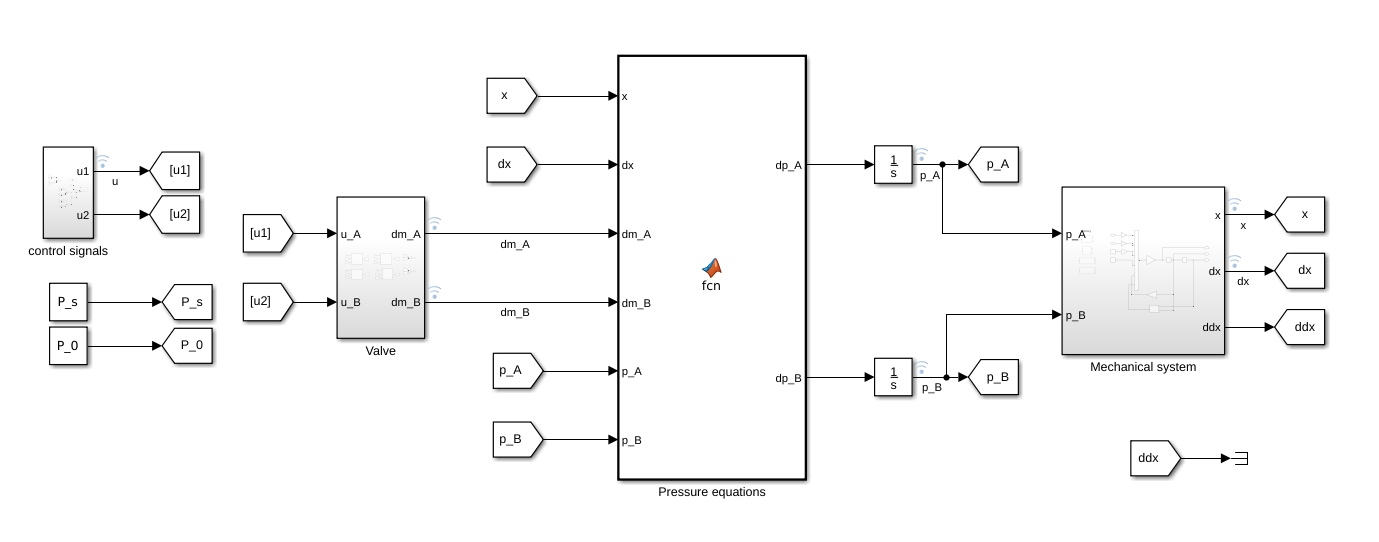
\includegraphics[width=1\textwidth]{equations.png}
    \caption{Simulink model based on equations}
    \label{fig:model_equations}
\end{figure}


\subsection{Model Simscape}
Model \ref{fig:model_simscape} was developed using SimScape toolbox.

\begin{figure}[h!]
    \centering
    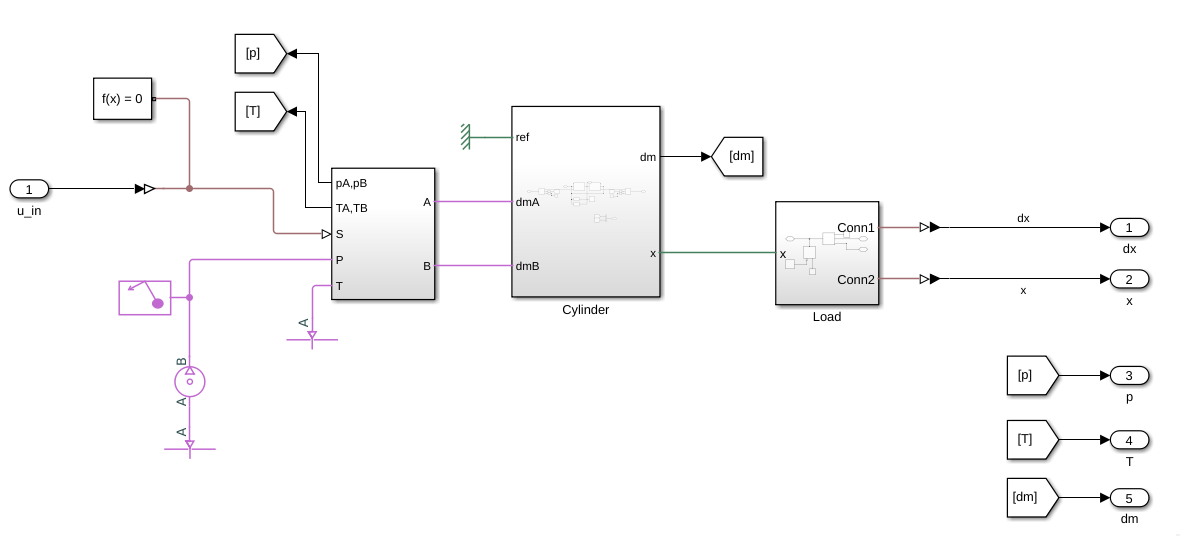
\includegraphics[width=1\textwidth]{simscape.png}
    \caption{Simulink model using SimScape Toolbox}
    \label{fig:model_simscape}
\end{figure}


\subsection{Comparison}
Following figure \ref{fig:compare_of_models} represent comparison of 2 models
(Simscape and based on equations) using same parameters for simulation:
There is slight difference between models causing Valve dynamics
simplifications in model based on equations.

\begin{figure}[h!]
    \centering
    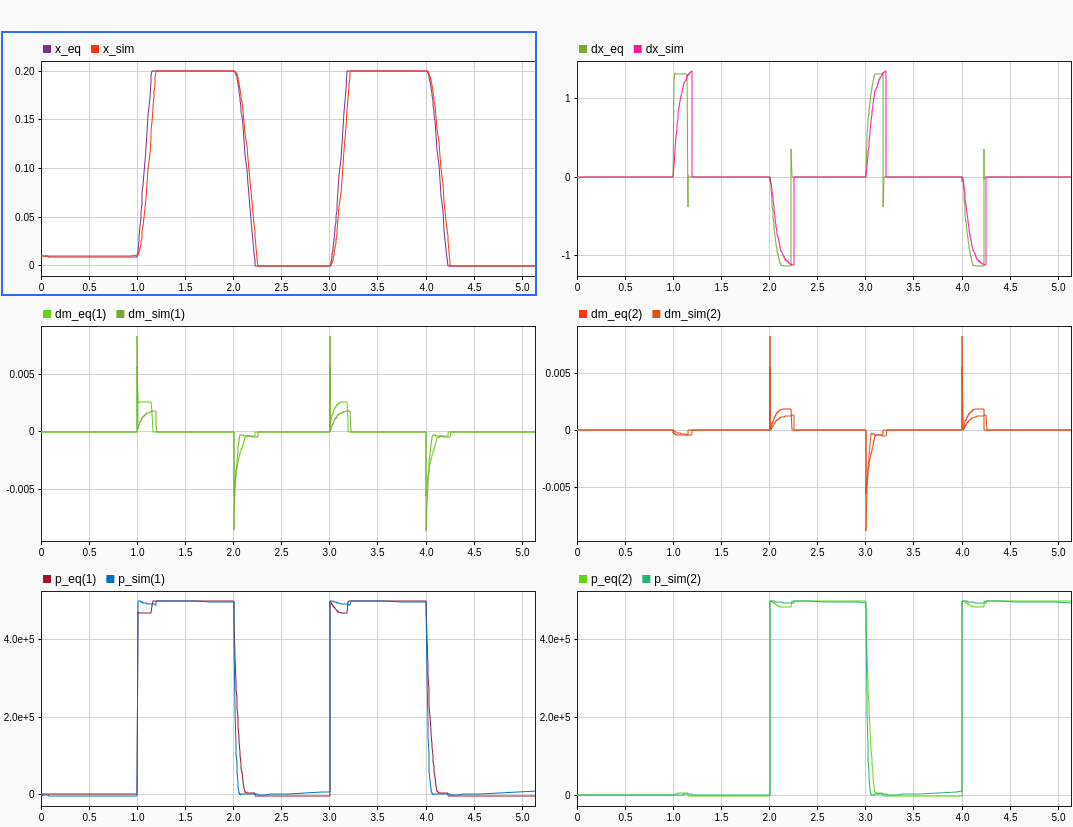
\includegraphics[width=1\textwidth]{models_comparation.png}
    \caption{Comparison of simscape and model based on equations}
    \label{fig:compare_of_models}
\end{figure}


\pagebreak
\section{Parameter identification}
\subsection{Mechanical assembly}
In mechanical system there is $F_f$ force represented by frictions accruing
in the system. This force can be modeled by different friction models with
respect to \ref{sec:mech_assembly}. Friction force parameters can be
estimated using "gray-box" method. 
Using $\dot{m}$ mass flow data versus $x$ position measured on real assembly
and use these data as an input and output, we can fit $F_f$.
Simplify model can contain TODO:
\begin{itemize}
    \item $F_C$ static friction
    \item $C_v$ viscous
    \item $C_p$ Pressure difference
\end{itemize}



\subsection{Cylinder}
Dead volume: $p_1 V_1^n = p_2 V_2^n$ or datasheet.

\subsection{Valve}
For valve system there are two parameters that need to be estimated.
According to equation \ref{eq:flow2} with constant $p_1$ (pressure supply) and $p_2$
(atmospheric pressure), we can estimate $\boldsymbol{C}$ if we neglect Valve Spool dynamic.
If in experiment we determine that spool dynamic necessary to include. We
provide same experiment with spool model including to "Gray-box" fitting
model.

\begin{align}
    \dot{m} = \boldsymbol{u}(x_s) \boldsymbol{C}  p_1 \sqrt{\frac{2}{RT_1}}
    \cdot \psi\left(\frac{p_2}{p_1}\right)
    \label{eq:flow2}
\end{align}

\end{document}

